\backgroundsetup{
  scale=1,
  opacity=0.6,
  angle=0,
  % contents={\includegraphics[width=\paperwidth]{images/bild.jpg}}
}

\begin{titlepage}
  \pagecolor{black}
  \color{white}

  \centering

  {\scshape\LARGE Maturaarbeit\par}
  \vspace{1cm}
  {\huge\bfseries Maschinelles Lernen mit TensorFlow\par}
  \vspace{0.2cm}
  {\large Entwicklung eines Convolutional Denoising Autoencoders\par}
  \vfill
  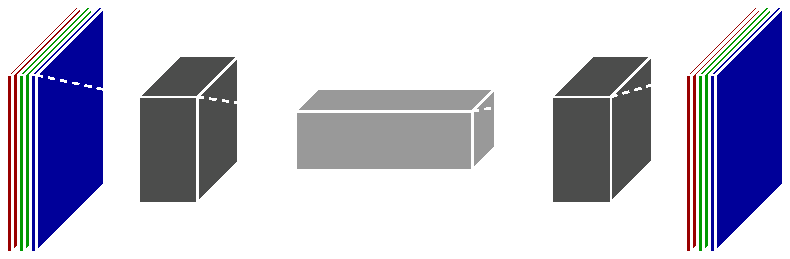
\includegraphics[width=0.9\textwidth]{titel.pdf} \par
  \vspace{1cm}
  {\Large\itshape Luis Wirth\par}
  \vfill
  \vspace{2cm}
  {\scshape\Large Gymnasium Oberwil\par}
  {\large Klasse \textit{4a}\par}
  \vspace{2cm}
  Betreut von\par
  Dr. Jonas \textsc{Gloor}

  \vfill
  {\large Abgegeben im September 2019\par}
\end{titlepage}

\pagecolor{pagecolor}
\color{textcolor}

\addcontentsline{toc}{chapter}{Inhaltsverzeichnis}
\tableofcontents

\pagebreak


\addcontentsline{toc}{chapter}{Vorwort}
\chapter*{Vorwort}
\section*{Persönliche Themenwahl}
Ich beschäftige mich schon seit geraumer Zeit mit Maschinellem Lernen und bin
sehr fasziniert von diesem Themengebiet. \\
Im Jahre 2017 habe ich bereits erste eigene Applikationen programmiert, welche
gebrauch von Machinellem Lernen machten. Damals habe ich einen Genetischen
Algorithmus geschrieben. \\
2018 habe ich die Möglichkeit erhalten ein Praktikum beim Departement für
Computational Physics zu machen. Dort durfte ich ein Künstliches Neuronales Netz
in C++ programmieren, welches ic hdann auf eine konkrete Physikalische
Problemstellung angewendet habe. Das Prkatikum hat mich dazu verleitet, mich
tiefgehdend mit Thema zu befassen und die grundlegende Funktionsweise von ML zu verstehen. \\
Diese Erfahrungen haben mich dazu inspiriert die vorliegende Arbeit zu schreiben.
Ich wollte mir durch diese Arbeit ein noch grundlegenderes mathematisches
Verstaentniss fuer Maschinelles Lernen aneignen und auch fortgeschritternere
Modelle betrachten. Desweiteren wusste ich von den begerten
Deep-Learning-Frameworks TensorFlow und Keras, welche ich schon lange einmal
lernen wollte zu verwenden. Somit versuchte ich mir eine passende Maturarbeit zu überlegen.
\para{}
Ich entschied mich einen Convolutional-Autoencoder in TensorFlow zu
programmieren und die nötige Theorie zu erklären. Ich wollte diesen Autoencoder
als ein generatives Modell verwenden um Bilder von künstlichen (erfundenen)
meschlichen Gesichtern zu generieren. \\
Im Verlauf der Arbeit musste ich jedoch feststellen, dass meine Arbeit anfing
den Rahmen einer Maturarbeit zu sprengen. Desweiteren habe ich simultan noch in
den Sommerferien ein 6-wöchiges Praktikum bei Adobe in San Francisco gemacht.
Auch dort habe ich ein Machine-Learning-Modell programmiert. Durch meine
praktikumsbezogenen Recherchen kam ich zur Erkenntnis, das meine Vorhaben mit
bezüglich der generativen Nutzung eines Autoencoder meine Resourcen übersteigen.
Ich hätte nämlich nicht nur einen Autoencoder programmieren müssen, sondern
sogar einen Variational Autoencoder. Dies wäre defintiv zu viel gewesen.
\para{}
Somit beschloss ich meine Leitfrage anzupassen. Ich beschränkte mich darauf
einen Convolutional \textit{Denoising} Autoencoder in TensorFLow und Keras zu
entwickeln und die nötige Theorie zu erklären.


\section*{Danksagung}
Ich möchte mich herzlich bei meiner Mutter Doris Fellenstein bedanken für das
Korrekturlesen und bei meiner Betreuungslehrperson, Jonas Gloor.


\addcontentsline{toc}{chapter}{Einleitung}
\chapter*{Einleitung}
Maschinelles Lernen ist schon seit längerer Zeit ein sehr heisser Themenbereich.
Er bitet unglaubliche Innovationspotential für die verschiedensten
Industriezweige. Selbstfahrende Autos, Google Assistent, Snapchat Filter; als
diese Technologien sind ein direktes Produkt vom Erfolg von Künstlicher
Intelligenz.
Interessante Aspekte: viele Anwendungszwecke von ML, Mathematik interesse
ALLGEMEINES ZUM THEMENGEBIET MACHINELLES LERNEN

INFORMATIONEN ZU DIESER ARBEIT: INHALT AUFBAU ETC
Das Ziel dieser Arbeit ist es, dem Leser ein umfangreiches Grundverstaentniss
ueber Maschinelles Lernen zu bieten. Dieses umfasst die theoretischen Grundlagen
zu modellbasiertem Lernen, Kuenstlichen Neuronalen Netzen, Convolutional Neural
Networks und Autoencodern. Mithilfe dieser erarbeiten Theorie wird dann noch die
die praktische Umsetzung eines Modells mithilfe von TensorFlow und Keras
erklaert. Bei TensorFlow und Keras handelt es sich um Frameworks fuer
Maschinelles Lernen mit Python. Sie sind in der Industrie sehr verbreitet und
wurden deshalb fuer diese Arbeit gewaehlt.
\para{}
Somit wurde die Leitfrage folgendermassen formuliert:
\textbf{Wie funktioniert Maschinelles Lernen und wie entwickelt man mit diesem
  Wissen ein konkretes Modell in TensorFlow?}
\para{}

Wir werden folgenden groben Aufbau verfolgen:

\begin{enumerate}
  \item{Wir erarbeiten die allgemeine Theorie zum Maschinellen Lernen.}
  \item{Wir betrachten Kuenstliche Neuronale Netze als Modelle fuer ML.}
  \item{Wir betrachten Convolutional Neural Networks und Autoencoder als
      konkrete KNN Architekturen.}
  \item{Wir betrachten die ML-Frameworks TensorFlow und Keras bezueglich ihrer Funktionsweise.}
  \item{Wir programmieren mithilfe der erarbeiten Theorie ein konkretes Modell
      in TensorFlow / Keras.}
\end{enumerate}

Für das konkrete Modell werden wir einen sogenannte
Convolutional-Denoising-Autoencoder entwickeln. In den Theorie Teilen werden wir
lernen wie dieser Funktioniert. Der Grund fuer die Wahl dieses konkreten Modells,
besteht darin, dass es sich dabei um ein Convolutional Neural Network handelt,
welche in den letzten Jahren sehr populär geworden sind und deshalb interessant
zu betrachten sind. Wir werden dieses Konzept eines Convolutional Neural Network
mit einem Autoencoder koppeln, um einen Convolutional-Denoising-Autoencoder zu
erhalten. Mithilfe von ihm können wir Bildrauschen von Bildern wegrechnen lassen.


\addcontentsline{toc}{chapter}{Konvention und Notation}
\chapter*{Konvention und Notation}

\subsection*{Beschriftung}

\begin{center}\textbf{Zahlen und Tensoren}\end{center}
\begin{tabular}{cl}
  $a$ & ein Skalar (Zahl) \\
  $\vec{a}$ & ein Vektor \\
  $\vec{a} \in \set{R}^{n}$ & ein Vektor mit $n$ Komponenten \\
  $\mat{A}$ & eine Matrix \\
  $\mat{A} \in \set{R}^{m \times n}$ & eine Matrix mit $m$ Zeilen und $n$ Spalten \\
  $\ten{A}$ & ein Tensor \\

\end{tabular}

\begin{center}\textbf{Mengen}\end{center}
\begin{tabular}{cl}
  $(a,b)$ & ein geordnetes Paar (2-Tupel) der Elemente $a$ und $b$ \\
  $\set{A}$ & eine Menge \\
  $\set{R}$ & die Menge aller reellen Zahlen \\
  $\set{Z}$ & die Menge aller ganzen Zahlen \\
  $\set{N}$ & die Menge aller natürlichen Zahlen \\
  $\{a,b\}$ & die Menge, welche aus den Elementen $a$ und $b$ besteht \\
  $\{1,\ldots,n\}$ & die Menge aller ganzen Zahlen von 1 bis $n$ \\
  $a \in \set{A}$ & $a$ ist ein Element der Menge $\set{A}$ \\

\end{tabular}

\begin{center}\textbf{Indexierung}\end{center}
\begin{tabular}{cl}
  $\vecelem{a}_i$ & die $i$-te Vektorkomponente mit Startindex 1 \\
  ${(\mat{A})}_{i,j}$ & das Matrixelement in der $i$-ten Zeile und der $j$-ten Spalte \\
  $\matelem{A}_{i,j}$ & das Matrixelement in der $i$-ten Zeile und der $j$-ten Spalte \\
  $\mat{A}_{i,:}$ & die Zeile $i$ der Matrix $\mat{A}$ \\
  $\mat{A}_{:,i}$ & die Spalte $i$ der Matrix $\mat{A}$\ \\
  $\ten{A}_{i,:,:}$ & der $i$-te Querschnitt entlang der Höhe des Tensors $\ten{A}$ \\
  $\ten{A}_{:,i,:}$ & der $i$-te Querschnitt entlang der Breite des Tensors $\ten{A}$ \\
  $\ten{A}_{:,:,i}$ & der $i$-te Querschnitt entlang der Tiefe des Tensors $\ten{A}$ \\
  $\mat{A} = \begin{pmatrix} \end{pmatrix}$ & Definition einer Matrix $\mat{A}$ \\
  $\ten{A} = \begin{bmatrix} \mat{A}_{:,:,1} & \cdots & \mat{A}_{:,:,c} \end{bmatrix}$ & Definition eines Tensors $\ten{A}$ \\

\end{tabular}

\begin{center}\textbf{Lineare Algebra Operationen}\end{center}
\begin{tabular}{cl}
  $\vec{v} \cdot \vec{w}$ & das Skalarprodukt von $\vec{v}$ mit $\vec{w}$ \\
  $\trans{\mat{A}}$ & das Transponierte einer Matrix $\mat{A}$ \\
  $\mat{A} \odot \mat{B}$ & das elementeweise (Hadamard) Produkt \\
  $\mat{A} * \mat{B}$ & die diskrete Faltung von $\mat{A}$ ueber $\mat{B}$

\end{tabular}

\begin{center}\textbf{Infinitesimalrechnung}\end{center}
\begin{tabular}{cl}
  $f'(x)$ & die Ableitung der Funktion $f$ bezüglich seinem Argument $x$ \\
  $\ds\deriv{y}{x}$ & die Ableitung von $y$ bezüglich $x$ \\[2ex]
  $\ds\partderiv{y}{x}$ & die partielle Ableitung von $y$ bezüglich $x$ \\[2ex]
  $\vecf{\nabla} y$ & der Gradient von $y$\\
  $\vecf{\nabla}_{\vec{x}}y$ & der Gradient von $y$ bezüglich $\vec{x}$ (Vektor) \\
  $\ds\int f(x)\,\text{d}x$ & das unbestimmte Integral der Funktion $f$ bezüglich $x$ \\
  $\ds\int_a^b f(x)\,\text{d}x$ & das bestimmte Integral der Funktion $f$ bezüglich $x$ von $a$ bis $b$ \\
  $\ds\lim_{x \to a} f(x)$ & der Limes/Grenzwert von $f$, wenn $x$ gegen $a$ strebt \\

\end{tabular}

\begin{center}\textbf{Funktionen}\end{center}
\begin{tabular}{cl}
  $f: \set{A} \to \set{B}$ & eine Funktion $f$ mit Definitionsmenge $\set{A}$ und Zielmenge $\set{B}$ \\
  $f(x)$ & eine Funktion $f$ mit Argument $x$ (Skalar) \\
  $f(\vec{v})$ & eine Funktion $f$ mit Argument $\vec{v}$ (Vektor) \\
  $\vecf{f}[\vec{v}]$ & die vektorisierte Funktion $\vecf{f}$ mit Argument $\vec{v}$ (Vektor) \\
  $\mathcal{A}$ & ein Funktionenraum \\
  $f * g$ & die Faltung von $f$ über $g$ \\
  $f \circ g$ & die Komposition von den Funktionen $f$ und $g$ \\

\end{tabular}

\begin{center}\textbf{Statistik}\end{center}
\begin{tabular}{cl}
  $\mathcal{N}$ & die Gauss'sche Normalverteilung \\
  $\phi$ & die Gauss'sche Dichtefunktion \\
  $\mu$ & der Erwartungswert/Mittelwert \\
  $\sigma^2$ & die Varianz
\end{tabular}

\begin{center}\textbf{Sonstiges}\end{center}
\begin{tabular}{cl}
  $\ds\sum_{i=a}^b x$ & die Summe mit von $a$ bis $b$ ueber $x$ mit Laufvariable $i$ \\
\end{tabular}

Erwähnung von Notation $\set{R}$ für Skalare und $\set{R}^n$ für Vektoren/Vektorräume...

%%% Local Variables:
%%% mode: latex
%%% TeX-master: "../main"
%%% End:
